\documentclass{article}

% packages
\usepackage[utf8]{inputenc}
\usepackage{pifont}
\usepackage{graphicx}
\graphicspath{{images/}}
\usepackage[hidelinks]{hyperref}
\usepackage{amsmath}
\usepackage{amssymb}
\usepackage{amsfonts}
\usepackage{mathtools}
\usepackage{xcolor}

\newcommand{\cmark}{\ding{51}}%
\newcommand{\xmark}{\ding{55}}%

% page format
\topmargin=-2cm
\textheight=23cm
\textwidth=19cm
\oddsidemargin=-1cm
\setlength{\parindent}{0pt}

\author{Guillaume W. Bres}
\title{zed-audio-dsp}

\begin{document}

\maketitle
\tableofcontents

\newpage
\section{System}

\begin{center}
	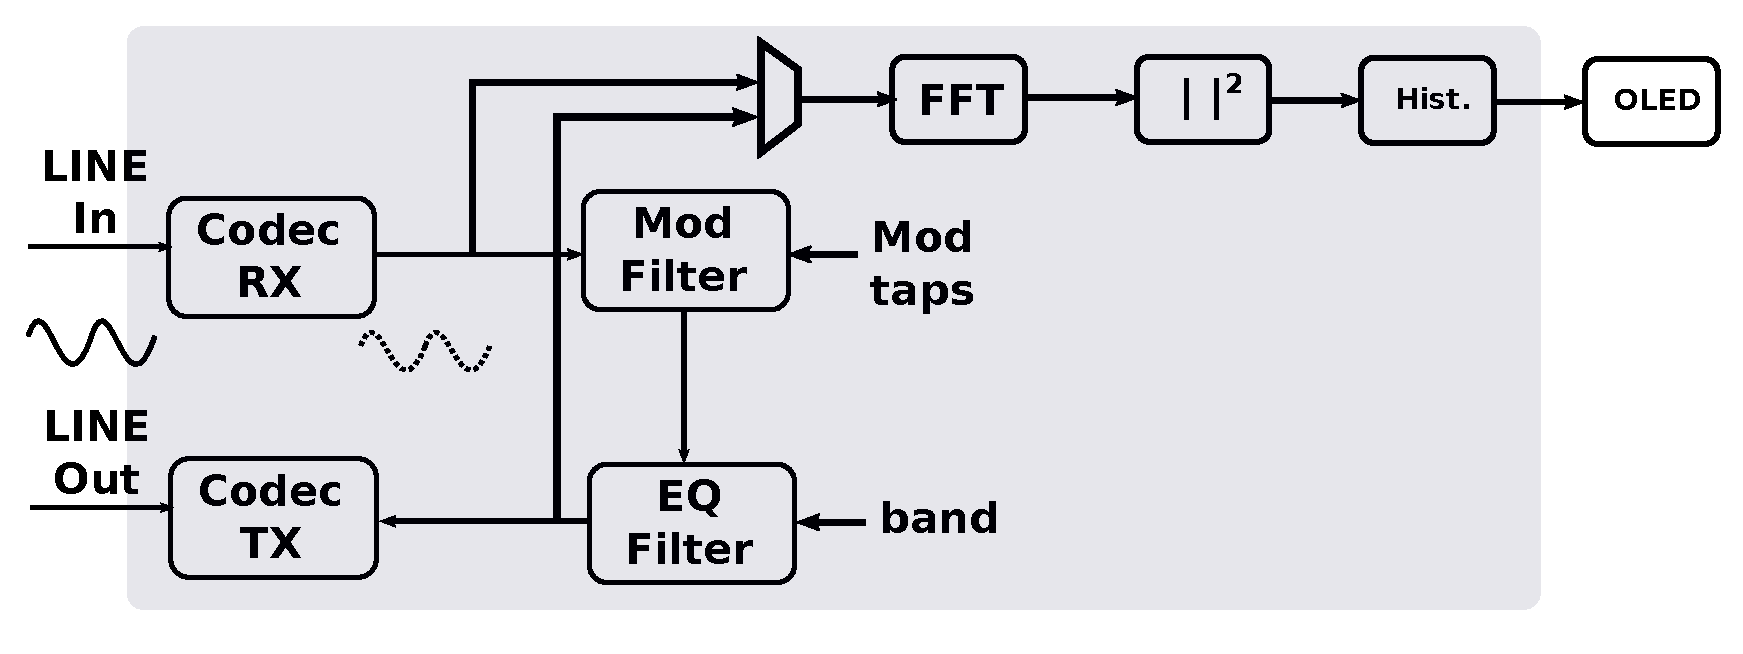
\includegraphics[width=0.75\linewidth]{bloc_design.pdf} \\
	Bloc design
\end{center}

All processing is real time and synchronous to the input
stream. The initial data rate is 1.152 Gb/s (much more than needed),
we reduce it to a 24 kHz (a little more than needed),
which means our internal rate is now 576 kB/s.
Data rate reduction is done using a CIC decimation filter. \\

The modulation filter as well as the
EQ filter are controlled from the User Interface. \\

The FFT processes either the
direct RX input or the output signal.
This allows to visualize the effect
of the modulation \& the EQ filters.
Switching is done in real time on user specs. \\

The resulting power spectrum is converted to histogram
\& displayed on the onboard OLED display.
The display is 128x32 pixel wide, which in our case
gives a spectral resolution of 187.5 Hz
on the display, which is more than decent.

The internal data stream obviously needs a final
interpolation, this is done by a CIC interpolation
filter, feeding a 1.152 Gb/s stream to the TX side.
The CIC interpolation filter is strictly symmetrical
to the CIC decimation filter.

\newpage
\subsection{CIC filters}

CIC filter being defined by $R, M, N$ parameters where

\begin{itemize}
	\item R: decimation/interpolation factor
	\item M: time delay, can either be 1 or 2 cycle
	\item N: number of stages
\end{itemize}

\vspace{0.2cm}
To reduce the initial rate from 1.152 Gb/s we fix
$R = 128$. \\

Both the interpolation \& decimation filters
are comprised of a N stages of integration filters
\& comb filters. \\

The {\tt \$git/dsp/cic.py} Python script 
can plot the frequency response
of a given CIC filter:

\begin{verbatim}
   $git/dsp/cic.py R=4 M=1 N=12
   $git/dsp/cic.py R=8 M=2 N=4
\end{verbatim}

%\begin{center}
%	\includegraphics[width=0.75\linewidth]{cic_filters.pdf} \\
%  Switching from a decimation to an interpolation is simply
%  changing the internal ordering and obviously performing
%  either a decimation or an interpolation in between
%  comb/integration stages.
%\end{center}

\begin{itemize}
	\item an integrator stage is defined as $H(z) = \frac{1}{1 - z^{-1}}$\\
	
	\item a comb stage is defined as $H(z) = 1 - z^{-M}$\\
	
	\item total CIC filter response is therefore $H(z) = \left| \frac{1 - z^-M}{1 - z^{-1}} \right|^N$
	
	\item the total magnitude response is approximated by
	$H(\nu) = \left| \frac{\sin(R M \pi \nu)}{R M \sin(\pi \nu)} \right|^N$

	\item the worst alias is encountered at frequency $\nu = \frac{3}{2MR}$
\end{itemize}

Increasing N (number of stages) increases the filter performance:

\begin{center}
	\begin{minipage}{0.49\linewidth}
		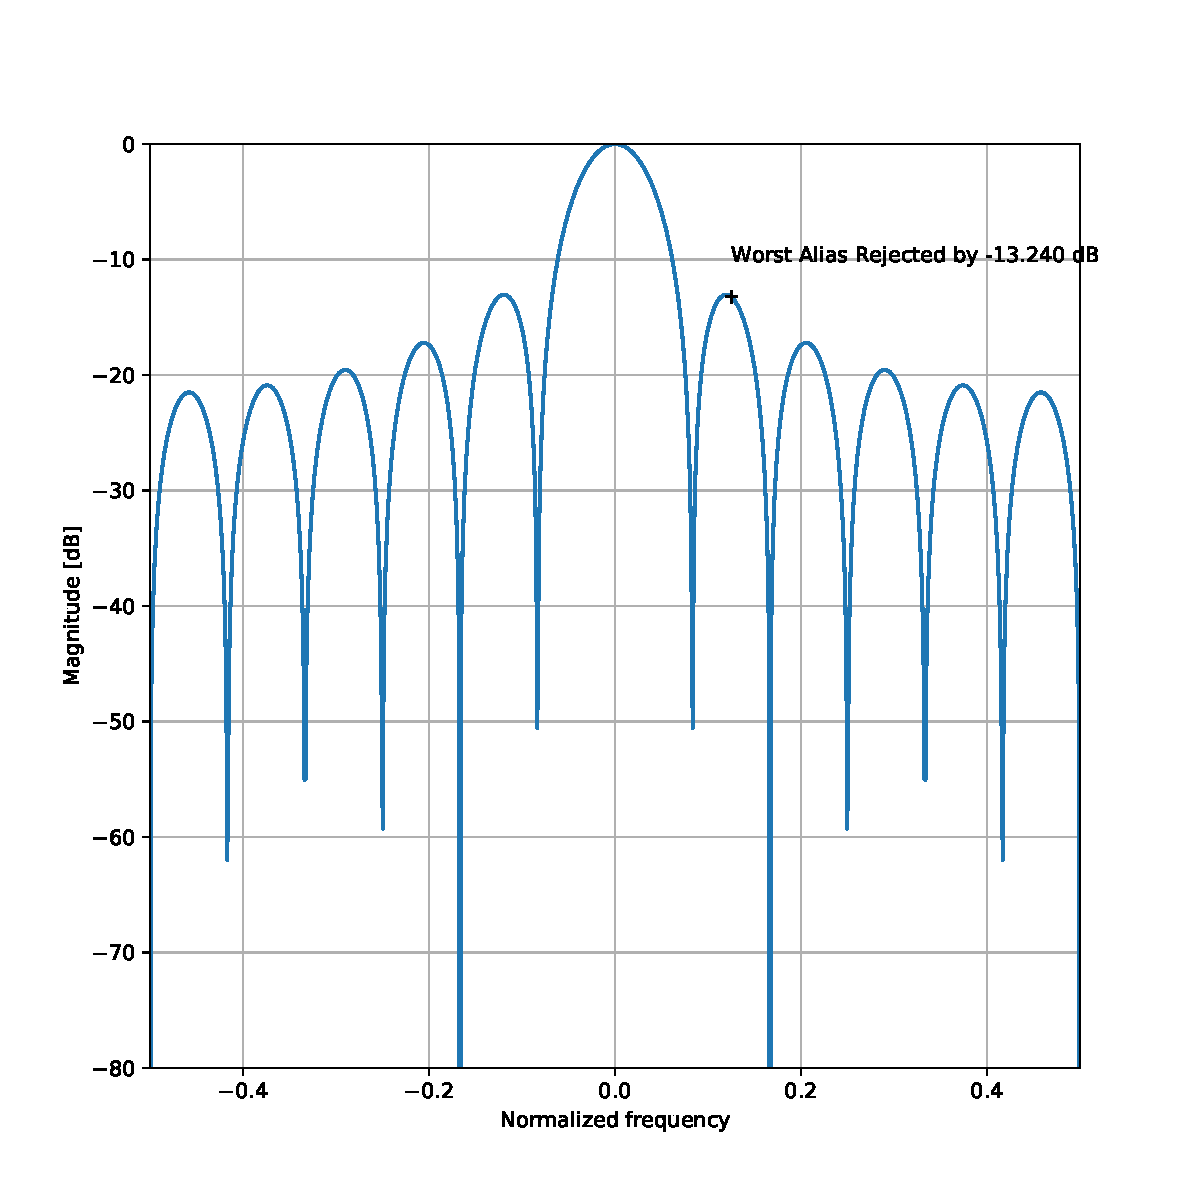
\includegraphics[width=0.99\linewidth]{cic_r12_n2.pdf} \\
		Comparing a CIC decimation filter with N=2 stages,
		the worst alias is rejected by -13 dB
	\end{minipage}
	\begin{minipage}{0.49\linewidth}
		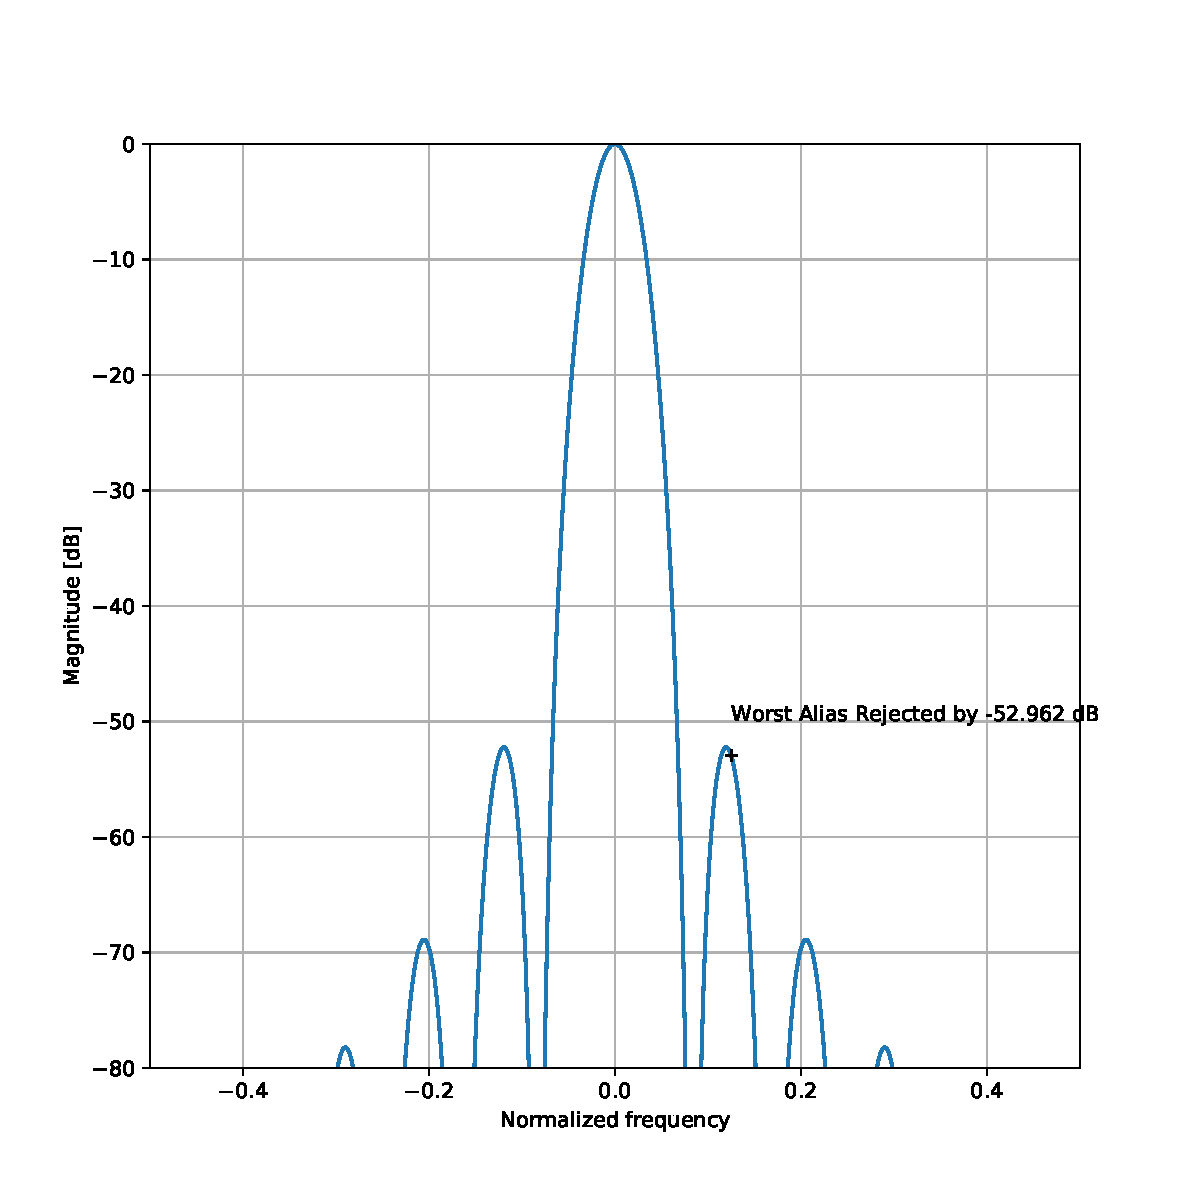
\includegraphics[width=0.99\linewidth]{cic_r12_n8.pdf} \\
		Increasing the number of stages to N=8
		improves the worst alias rejection to -53 dB
	\end{minipage}
\end{center}

We fix $N=8$ in our case, not to consume too much ressources.
This will give a rejection of
-53 dB for the worst alias ever encountered. \\

We introduce a compensation filter (in the form of an FIR
filter) to compensate for the  $f(\nu) = \frac{sin(\nu)}{\nu}$ shape
of the CIC frequency response (as seen in previous plot). \\

If we do not compensator for the CIC response, the entire bandwidth
becomes almost unusable. \\

The compensation filter response is the exact inverse
of the CIC filter response $G(z) = \frac{1}{H(z)}$ 
in the output frequency domain. \\

\subsection{CIC compensation filter}

The CIC compensation filter is designed
using the python script {\tt \$git/dsp/cic-compensator.py}. 

\begin{verbatim}
   $git/dsp/cic-compensator.py R=4 M=1 N=12
   $git/dsp/cic-compensator.py R=8 M=2 N=4
\end{verbatim}

CIC filter compensation 
will be implemented in both the decimation
\& the interpolation filter, using
Xilinx's optimized FIR filter IP core. \\

\subsection{FFT Histogram}

The Histogram IP core converts
the power spectrum from the

\subsection{CIC compensation filter}

The CIC compensation filter is designed
using the python script {\tt \$git/dsp/cic-compensator.py}. 

\begin{verbatim}
   $git/dsp/cic-compensator.py R=4 M=1 N=12
   $git/dsp/cic-compensator.py R=8 M=2 N=4
\end{verbatim}

\subsection{FFT Histogram}

The Histogram IP core converts
the power spectrum from the
magnitude IP core
to a histogram to be displayed on the OLED. \\

It is a simple mapping of the resulting
power spectrum to a 2D array (X,Y) describing
the power spectrum along a frequency axis. \\ 

%\begin{center}
%	\includegraphics[width=0.75\linewidth]{fft_histogram.pdf} \\
%\end{center}

\section{Simulation}

Install {\tt ghdl} to easily
simulate modules that come with a testbench:

\begin{verbatim}
git clone https://github.com/ghdl/ghdl
cd ghdl
./configure
make
sudo make install
\end{verbatim}

Once this is done, you can safely simulate a module
that comes with a testbench by using {\it make}
in its {\tt sim} folder.
For example:

\begin{verbatim}
cd $git/ip/adau1761/sim
make
\end{verbatim}

\end{document}
